\documentclass{article}


%%%%%%%%%%%%%%%%%%%%%%%%%%%%%%%%%%%%%%%%%%%%%%%%%%%%%%%%%%%%%%%%%%%%%%%%%
\pagestyle{plain}                                                      %%
%%%%%%%%%% EXACT 1in MARGINS %%%%%%%                                   %%
\setlength{\textwidth}{6.5in}     %%                                   %%
\setlength{\oddsidemargin}{0in}   %% (It is recommended that you       %%
\setlength{\evensidemargin}{0in}  %%  not change these parameters,     %%
\setlength{\textheight}{8.5in}    %%  at the risk of having your       %%
\setlength{\topmargin}{0in}       %%  proposal dismissed on the basis  %%
\setlength{\headheight}{0in}      %%  of incorrect formatting!!!)      %%
\setlength{\headsep}{0in}         %%                                   %%
\setlength{\footskip}{.5in}       %%                                   %%
%%%%%%%%%%%%%%%%%%%%%%%%%%%%%%%%%%%%                                   %%
\newcommand{\required}[1]{\section*{\hfil #1\hfil}}                    %%
\renewcommand{\refname}{\hfil References Cited\hfil}                   %%
\bibliographystyle{plain}                                              %%
%%%%%%%%%%%%%%%%%%%%%%%%%%%%%%%%%%%%%%%%%%%%%%%%%%%%%%%%%%%%%%%%%%%%%%%%%

\usepackage{graphicx}

\pagestyle{empty}

\begin{document}

\large

\vbox{}
\begin{figure}[!ht]
%\hspace{-4mm}

\includegraphics[width=8cm]{img/logo.png}
\vspace{12mm}
\end{figure}

\begin{figure}[!ht]
\begin{center}
%\hspace{-4mm}
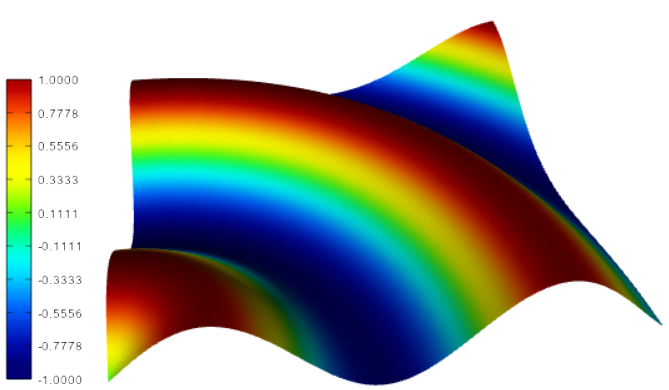
\includegraphics[width=14cm]{img/webgl.png}
\vspace{16mm}
\end{center}
\end{figure}

\centerline{\Huge \bf NCLab as a Graphing Calculator}

\vfill

\centerline{\Large www.nclab.com}

\newpage

%%%%%%%%%%%%%%%%%%%%%%%%%%%%%%%%%%%%%%%%%%%%%%%%%%%%%%%%%%%%%%%%%%%%%%%%%



\section*{}
\small
\input ../common/aboutnclab.tex

%\subsection*{Acknowledgement}
%This publication was created with the help of numerous freely 
%available web resources and tutorials related to Python, Scipy,
%Numpy, Pylab, Matplotlib, Sympy and other projects.

\normalsize

\newpage
%{\ }
\setcounter{tocdepth}{2}
\tableofcontents
%\pagestyle{plain}

\newpage

\pagestyle{plain}
\setcounter{page}{1}


%%%%%%%%%%%%%%%%%%%%%%%%%%%%%%%%%%%%%%%%%%%%%%%%%%%%%%%%%%%%%%%%%%%%%%%%%
\newpage

\pagestyle{plain}


\section{Introduction}

The advantage of simple calculators, such as the one shown in Fig. \ref{fig:xcalc}
is that they only have a few functions, and thus can be operated using a few buttons.

\begin{figure}[!ht]
\begin{center}
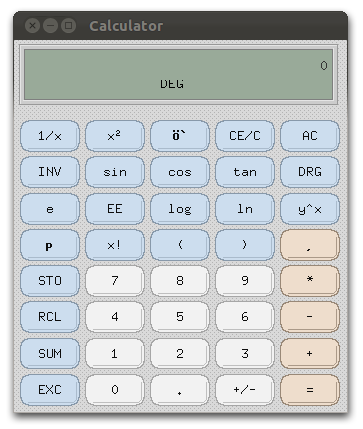
\includegraphics[width=0.4\textwidth]{img/xcalc.png}
\end{center}
%\vspace{-2mm}
\caption{Simple calculator.}
\label{fig:xcalc}
\end{figure}
\noindent
Compared to this calculator, NCLab provides an enormous functionality 
that would require hundreds of buttons. So instead of buttons,
in NCLab we use simple commands to get the results we want. The language used 
to talk to NCLab is called Python. Using Python is very intuitive, 
as we shall see in a moment.

\section{Launching a Python Project}

Python worksheet can be launched through the File Manager or through 
the Programming icon on Desktop. Let's do for example the latter. 
This will lanuch a new Python worksheet, as illustrated in Fig. 
\ref{fig:python}. 

\newpage

\begin{figure}[!ht]
\begin{center}
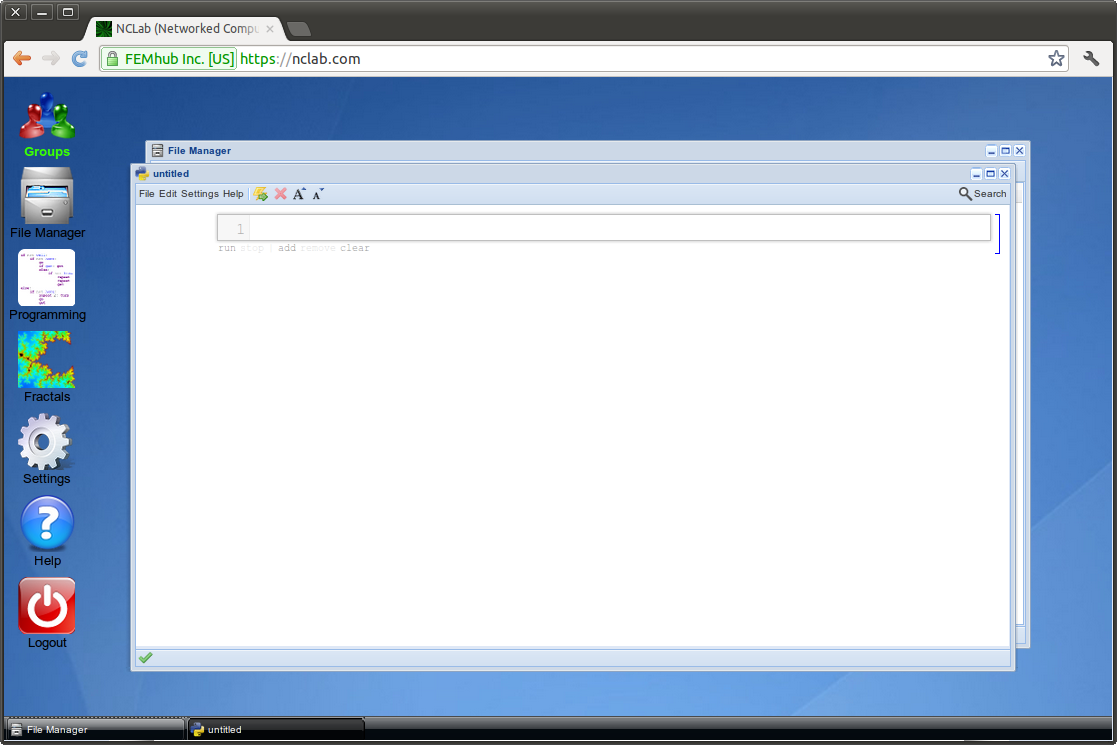
\includegraphics[width=\textwidth]{img/python.png}
\end{center}
%\vspace{-2mm}
\caption{Python worksheet.}
\label{fig:python}
\end{figure}
\noindent

\section{Cloning Displayed Projects}

All examples that we are going to work with in the following are also available 
as Displayed Projects. This means that you can clone them by going to the
File Manager's Project menu and clicking on {\em Clone}. This will launch 
a window with many displayed projects from various areas of programming,
math and computing. Look for projects titled such as "Math - Tutorial - 1 - Simple Arithmetic",
"Math - Tutorial - 2 - Commutative, Associative and Distributive Laws", etc.
After you locate a project that you would like to clone, click on it,
and then click on the button "Clone" at the bottom of the window. This will
create exact copy of that project in your account, and you can open it 
by clicking on it in the File Manager. You can change the project in any way 
you like, the changes will not affect the original Displayed Project. 

\section{Simple Arithmetic}

Let's say that we have not cloned the displayed project "Math - Tutorial - 1 - Simple Arithmetic"
and instead, we prefer to start from scratch.
So your project contains a single {\em input cell}. Let's write 
something simple into it, for example "1 + 2", and click 
the link "run" right under the input cell. This sends a request to 
the cloud, it is processed there, and an answer comes back instantly. 
It is displayed in a new (yellow) {\em output cell}, as shown in 
Fig. \ref{fig:1p3}.

\begin{figure}[!ht]
\begin{center}
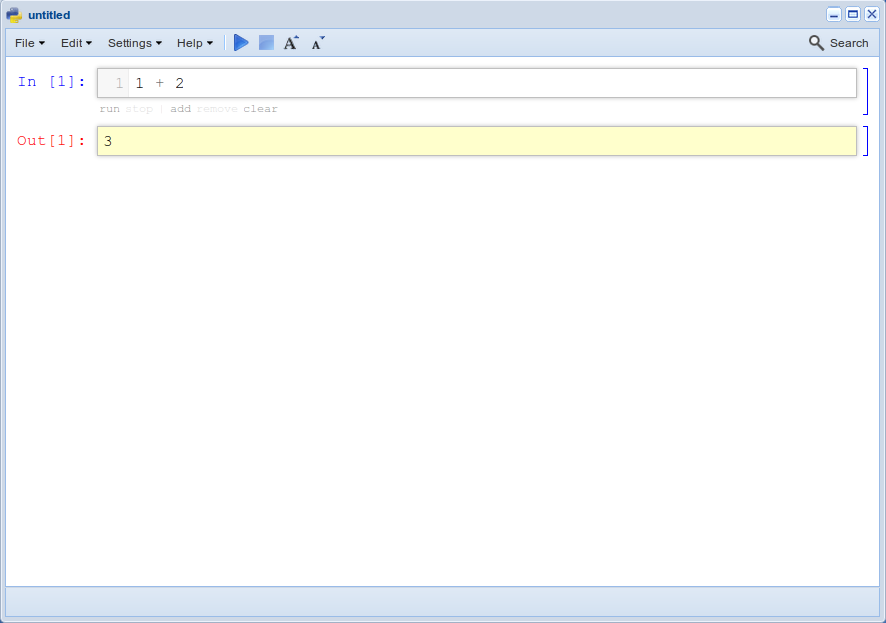
\includegraphics[width=\textwidth]{img/1p2.png}
\end{center}
%\vspace{-2mm}
\caption{Evaluating the expression "1+2".}
\label{fig:1p3}
\end{figure}
\noindent
\noindent
In addition to input and output cells, you can use {\em text cells}
to keep your project commented. This is strongly recommended. In
order to add a new text cell above the input cell, click into
the input cell, and then in menu Edit choose "New text cell above
active cell". A new text cell appears, asking you to click there to
edit its contents. Do so, and write, for example, "**Adding numbers**".
The double stars are used to make a text between them bold face. 
Then click on the link "save" right under the text cell. The result 
is shown in Fig. \ref{fig:1p3r}.

\newpage


\begin{figure}[!ht]
\begin{center}
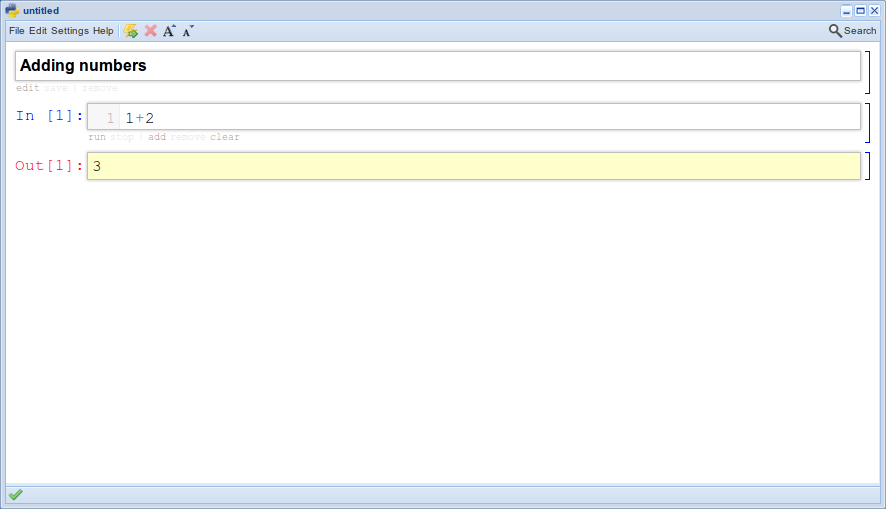
\includegraphics[width=\textwidth]{img/1p3r.png}
\end{center}
%\vspace{-2mm}
\caption{New descriptive text cell was added above the input cell.}
\label{fig:1p3r}
\end{figure}
\noindent
\noindent
If you like, you can click back into the input cell, change 
the numbers, and click the "run" link under the cell again. 
This will send a new request to the cloud and after the answer 
comes back, it is displayed in the existing output 
cell. 

Let's continue by creating a new empty input cell. To do this, click 
on the "add" below the last input cell. The new input cell will appear below the yellow 
output cell (it will never be placed between an input cell and its 
result). In there, we can experiment with other arithmetic operations 
including subtraction (try for example "5 - 3"), multiplication 
(try for example "3.21 * 7.45"). The results are shown in Fig. \ref{fig:1p3r2}.

\newpage

\begin{figure}[!ht]
\begin{center}
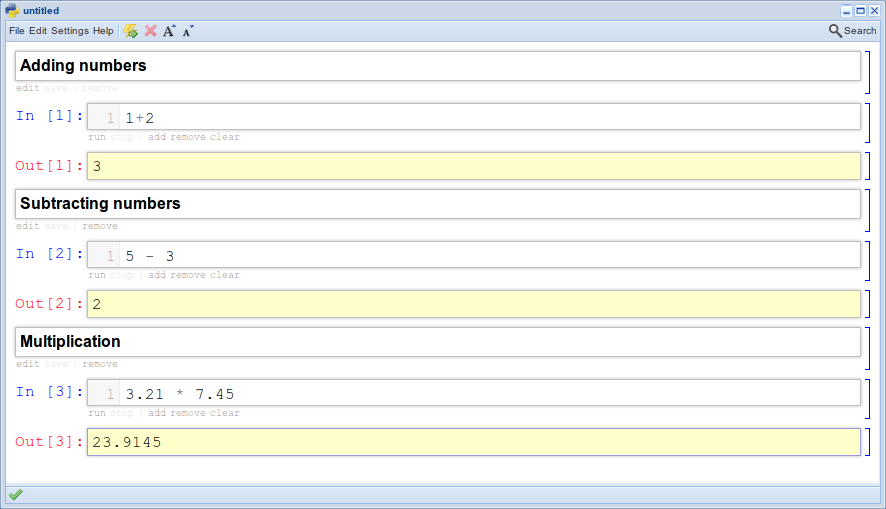
\includegraphics[width=\textwidth]{img/1p3r2.png}
\end{center}
%\vspace{-2mm}
\caption{Subtraction and multiplication.}
\label{fig:1p3r2}
\end{figure}
\noindent
At this point we may go to menu Edit and click on 
"Remove all output" -- this will free up some space.\\

\noindent
{\em BEWARE - Division of Two integers Always is an Integer}\\

Numbers such as "12" or "5" are integers. In Python, as well as 
in other major programming languages, the {\bf result of division of 
two integers always is an integer}. This means that anything beyond 
the decimal point in the result is erased! Let us see this in reality:

\newpage
\begin{figure}[!ht]
\begin{center}
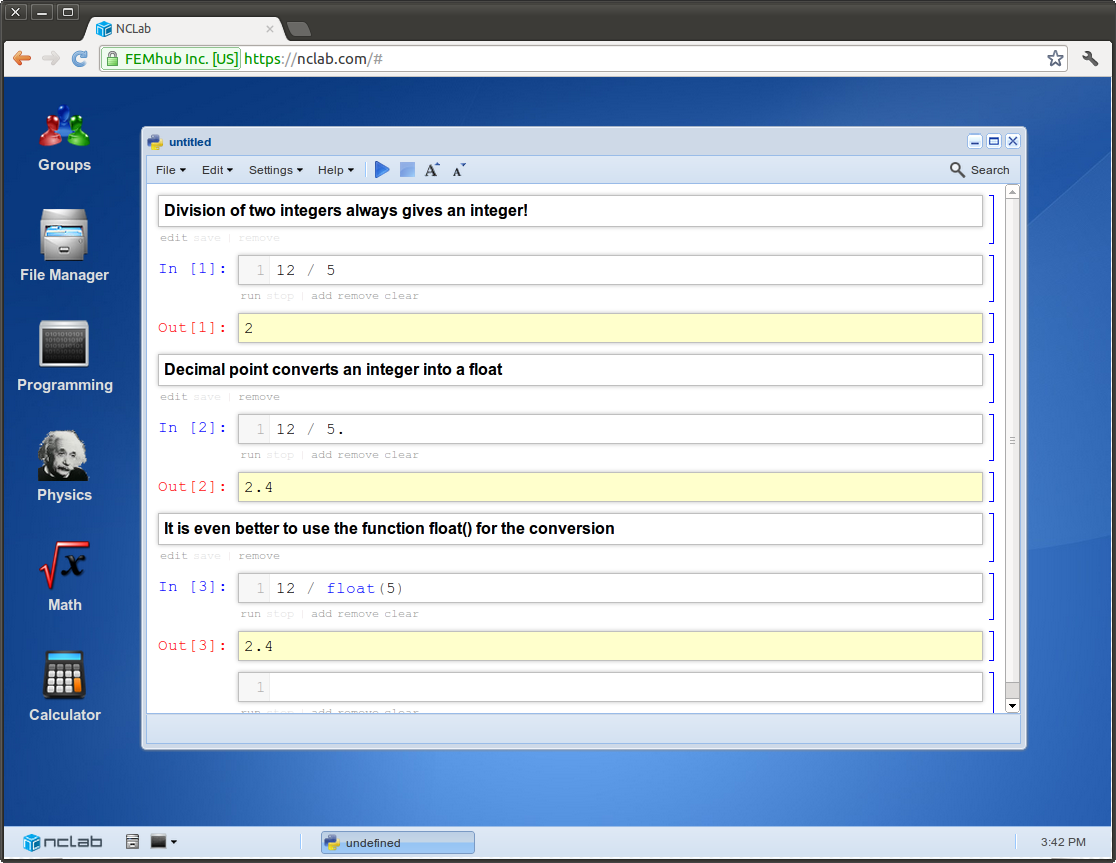
\includegraphics[width=\textwidth]{img/div1.png}
\end{center}
%\vspace{-2mm}
\caption{Division of two integers always is an integer \& two ways to make division safe.}
\label{fig:div1}
\end{figure}
\noindent
Fig. \ref{fig:div1} shows that evaluating simply 12/5 leads to a wrong result. An easy fix is 
to convert one of the numbers into a float by appending a decimal point to it. Still
another way, also shown in  Fig. \ref{fig:div1}, is to convert one of the numbers into a float 
via the function {\tt float()}. The latter approach works even for the division of variables "a/b"
where one may not know exactly whether they are integers or floats. Whenever at least 
one of the numbers if float, the result is a float. \\

\noindent
If you are a mathematician -- yes, you are right. we forgot to discuss division by zero. 
It is useful to see how NCLab reports errors, so let's do it!

\newpage
\begin{figure}[!ht]
\begin{center}
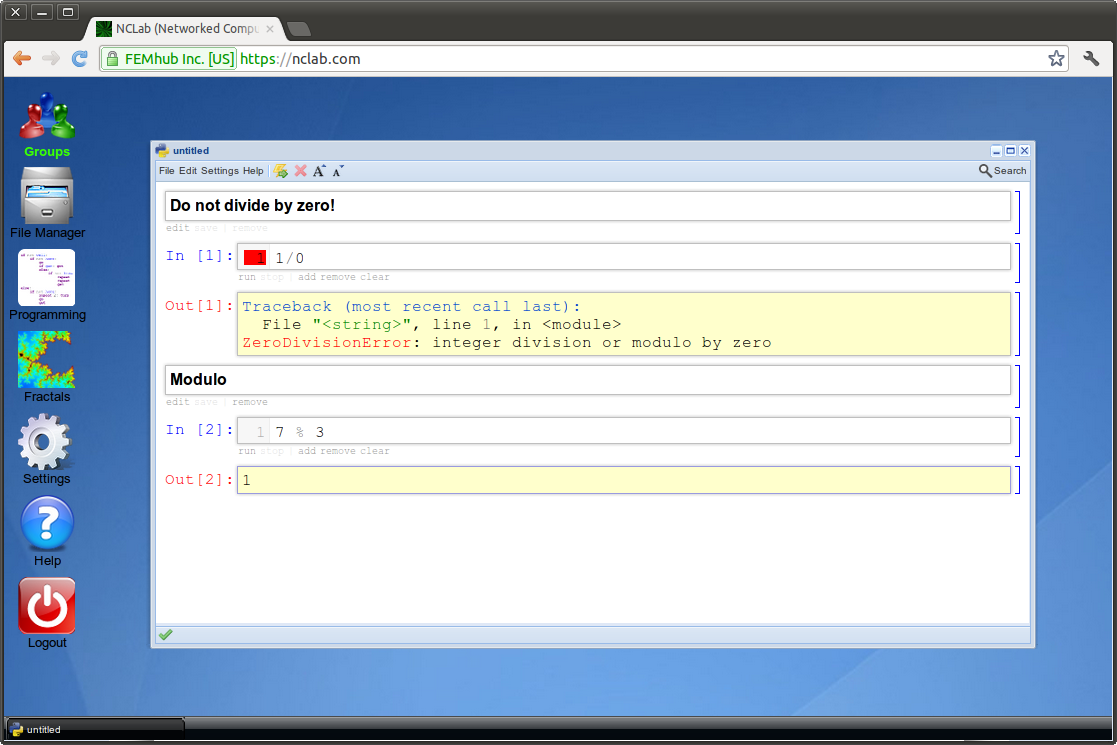
\includegraphics[width=\textwidth]{img/divzero.png}
\end{center}
%\vspace{-2mm}
\caption{Error is reported when dividing by zero.}
\label{fig:divzero}
\end{figure}
\noindent
Since the error message in Fig. \ref{fig:divzero} mentioned modulo, we added there one more 
input cell demonstrating how modulo is done -- using the \% symbol.

\section{List of Elementary Functions}

In order to calculate square roots, exponentials, sins, cosins, tangents, and all other 
simple functions, the best way is to import Numpy as shown in Fig. \ref{fig:fns}. Numpy 
is a standard Python library for numerical computations.

\begin{figure}[!ht]
\begin{center}
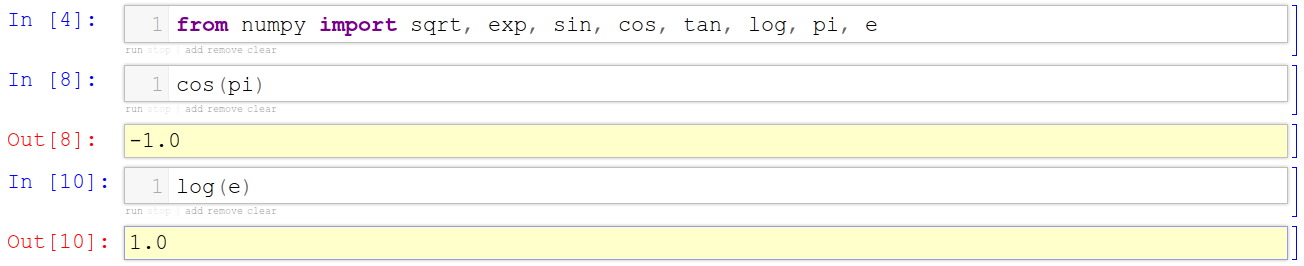
\includegraphics[width=\textwidth]{img/fns.png}
\end{center}
\vspace{-4mm}
\caption{Importing Numpy and using elementary functions.}
\label{fig:fns}
%\vspace{-6mm}
\end{figure}

\newpage
\noindent
Elementary functions that one can import from Numpy include:\\

%{\small
\begin{center}
\begin{tabular}{|l|l|}
\hline
abs($x$) &  absolute value of $x$\\
arccos($x$) &  inverse cosine of $x$ \\
arccosh($x$) &  inverse hyperbolic cosine of $x$ \\
arcsin($x$) & inverse sine of $x$ \\
arcsinh($x$) & inverse hyperbolic sine of $x$ \\
arctan($x$) & inverse tangent of $x$ \\
arctanh($x$) & inverse hyperbolic tangent of $x$ \\
arctan2($x_1$, $x_2$) & arc tangent of $x_1/x_2$ choosing the quadrant correctly \\
cos($x$) & cosine of $x$ \\
cosh($x$) & hyperbolic tangent of $x$ \\
exp($x$) & $e^x$ \\
log($x$) & natural logarithm of $x$ \\
pow($a$, $b$) & $a^b$ (same as "a**b")\\
sin($x$) & sine of $x$ \\
sinh($x$) & hyperbolic sine of $x$ \\
sqrt($x$) & square root of $x$ \\
tan($x$) & tangent of $x$\\
tanh($x$) & hyperbolic tangent of $x$ \\
\hline
\end{tabular}
\end{center}
%}
\vspace{4mm}
\noindent
For a complete overview of functions provided by Numpy we recommend the 
web page \\ {\tt http://www.scipy.org/Numpy\_Functions\_by\_Category}.

%%%%%%%%%%%%%%%%%%%%%%%%%%%%%%%%%%%%%%%%%%%%%%%%%%%%%%%%%%%%%%%%%%%%%%%%

\section{Plotting functions of one variable}\label{plotting}

Plotting can be done via the Pylab library. The Pylab {\tt plot} command takes two
arrays: $x$-coordinates and $y$-coordinates of points on a curve. Between the 
points, the curve is interpolated linearly. Let us illustrate this on a simple 
example with just five points [0, 0], [1, 2], [2, 0.5], [3, 2.5] and [4, 0]:

\begin{verbatim}
from pylab import *
x = [0,0, 1.0, 2.0, 3.0, 4.0]
y = [0.0, 2.0, 0.5, 2.5, 0]
clf()
plot(x, y)
lab.show()
\end{verbatim}
The commands {\tt clf()}, {\tt plot()} and {\tt lab.show()} do clear the canvas, 
plot the graph, and show the graph, respectively.
The output is shown in Fig. \ref{fig:plot}.
\newpage

\begin{figure}[!ht]
\begin{center}
\hbox{}
\hspace{-6mm}
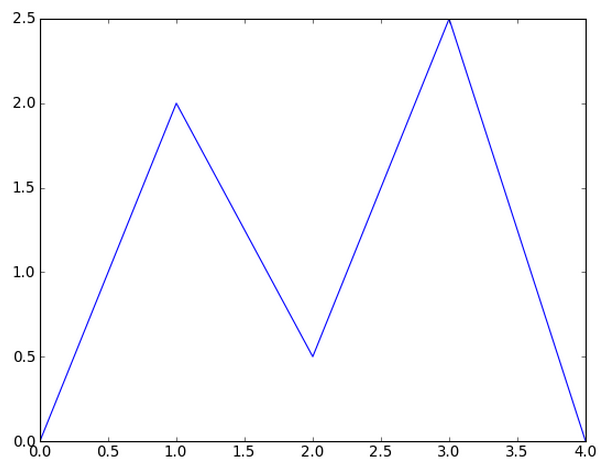
\includegraphics[width=0.56\textwidth]{img/plot.png}
\end{center}
\vspace{-2mm}
\caption{Piecewise-linear curve with five points.}
\label{fig:plot}
%\vspace{-1cm}
\end{figure}
\noindent
In the following we will discuss more options and show some useful techniques.
Let's say, for example, that we want to plot the function $f(x) = \sin(x)$
in the interval $(0, 2\pi)$. The array of $x$-coordinates of equidistant points 
between 0 and $\pi$ with step 0.05 can be created easily using the command {\tt arange}:

\begin{verbatim}
from numpy import *
x = arange(0, 2*pi, 0.05)
\end{verbatim}
Changing the step size will change the resolution - with a smaller step the resolution will 
be finer and vice-versa. Next, the array of $y$-coordinates of the points is obtained via

\begin{verbatim}
y = sin(x)
\end{verbatim}
The last part we already know:

\begin{verbatim}
clf()
plot(x, y)
lab.show()
\end{verbatim}
\noindent
The output is shown in Fig. \ref{fig:plot1}.
\newpage

\begin{figure}[!ht]
\begin{center}
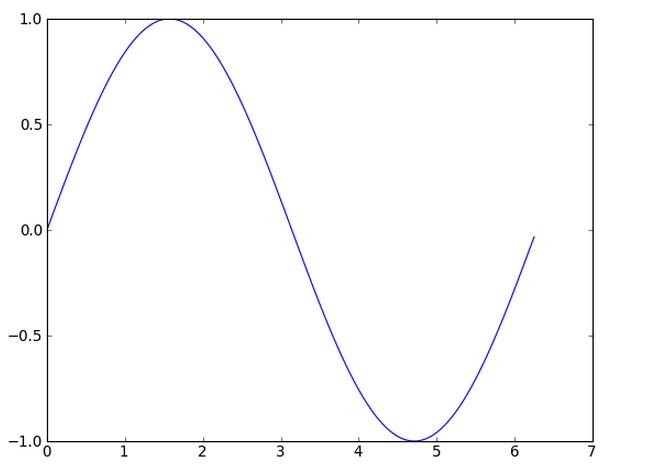
\includegraphics[width=0.6\textwidth]{img/plot1.png}
\end{center}
\vspace{-6mm}
\caption{Plotting $\sin(x)$ in interval $(0, 2\pi)$ with subdivision step 0.05.}
\label{fig:plot1}
\vspace{-2mm}
\end{figure}
\noindent

\section{Labels, colors, and styles}

The plot can be made nicer by adding a label, and also the color 
and the line style can be changed. Let us start with adding a label:

\begin{verbatim}
plot(x, y, 'b-', label = "Solid blue line")
legend()
lab.show()
\end{verbatim}
The output is shown in Fig. \ref{fig:plot2}.

\begin{figure}[!ht]
\begin{center}
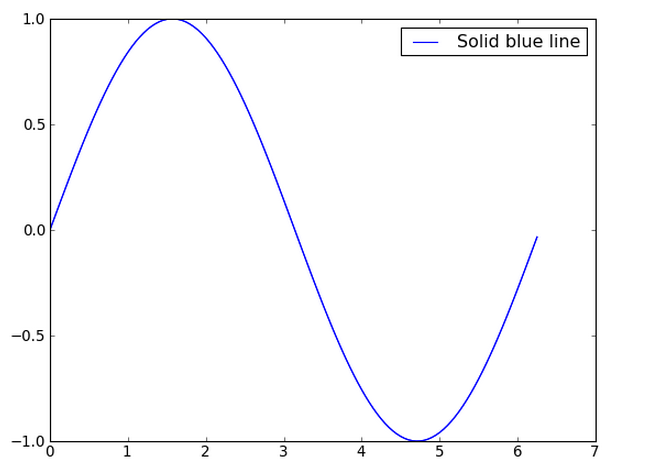
\includegraphics[width=0.6\textwidth]{img/plot2.png}
\end{center}
\vspace{-6mm}
\caption{Adding a label.}
\label{fig:plot2}
%\vspace{-1cm}
\end{figure}
\newpage
\noindent
Next let us change the color to red and line style to dashed: 

\begin{verbatim}
clf()
plot(x, y, 'r--', label = "Dashed red line")
legend()
lab.show()
\end{verbatim}
The output is shown in Fig. \ref{fig:plot3}.

\begin{figure}[!ht]
\begin{center}
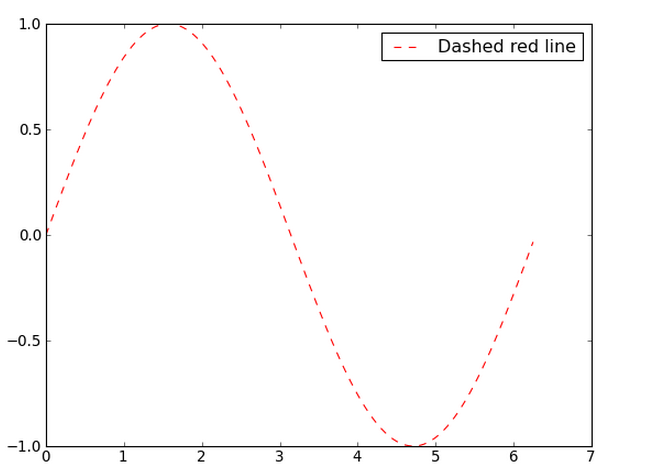
\includegraphics[width=0.6\textwidth]{img/plot3.png}
\end{center}
\vspace{-6mm}
\caption{Same graph using dashed red line.}
%\vspace{-4mm}
\label{fig:plot3}
\end{figure}
\noindent
The graph can be plotted using green color and small dots rather than 
a solid or dashed line:

\begin{verbatim}
clf()
plot(x, y, 'g.', label = "Dashed red line")
legend()
lab.show()
\end{verbatim}
The output is shown in Fig. \ref{fig:plot4}.
\newpage

\begin{figure}[!ht]
\begin{center}
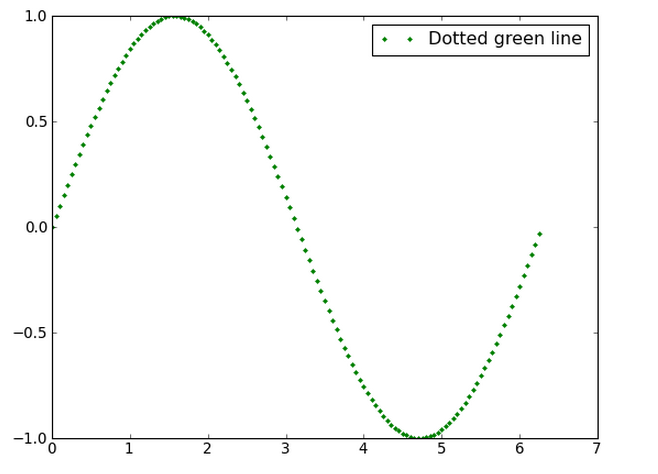
\includegraphics[width=0.6\textwidth]{img/plot4.png}
\end{center}
\vspace{-6mm}
\caption{Same graph using dotted green line.}
\label{fig:plot4}
%\vspace{-5mm}
\end{figure}
\noindent
Last let us stay with green color but make the dots larger:

\begin{verbatim}
clf()
plot(x, y, 'go', label = "Dashed red line")
legend()
lab.show()
\end{verbatim}
\noindent
The output is shown in Fig. \ref{fig:plot5}.

\begin{figure}[!ht]
\begin{center}
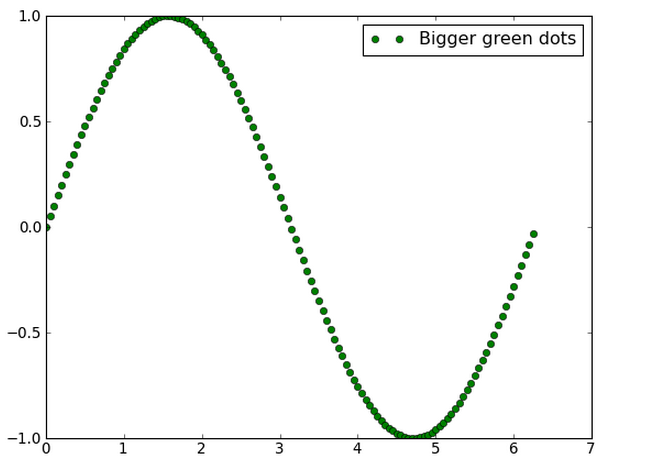
\includegraphics[width=0.6\textwidth]{img/plot5.png}
\end{center}
\vspace{-6mm}
\caption{Same graph using large green dots.}
\label{fig:plot5}
%\vspace{-4mm}
\end{figure}
\noindent

\section{Scaling axes and showing grid}

In the previous plots, the function graphs were fitted into the 
display window, which means that the horizontal and vertical 
exas were scaled differently. This can be changed by including the 
{\tt axis('equal')} command after calling {\tt plot()}. Also, 
grid can be displayed by using the {\tt grid()} command:

\begin{verbatim}
from numpy import *
from pylab import *
x = arange(0, 2*pi, 0.05)
y = sin(x)
clf()
plot(x, y, label="sin(x)")
axis('equal')
grid()
legend()
lab.show()
\end{verbatim}
\noindent
The output is shown in Fig. \ref{fig:plot8}.

\begin{figure}[!ht]
\begin{center}
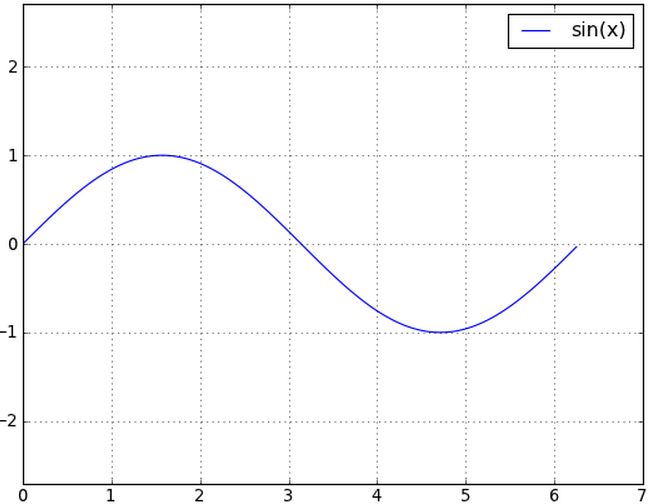
\includegraphics[width=0.53\textwidth]{img/plot8.png}
\end{center}
\vspace{-4mm}
\caption{Scaling axes equally and showing grid.}
\label{fig:plot8}
\end{figure}
\noindent
The scaling of axes can be returned to the automatic fit option via
{\tt axis('auto')} if needed.

\section{Adjusting plot limits}

Plot limits can be set using the {\tt xlim()} and {\tt ylim()}
functions after {\tt plot()}. For example, we can stretch the sine
function from Fig. \ref{fig:plot8} to span the entire width of the 
canvas as follows:

\begin{verbatim}
from numpy import *
from pylab import *
x = arange(0, 2*pi, 0.05)
y = sin(x)
clf()
plot(x, y, label="sin(x)")
xlim(0, 2*pi)
axis('equal')
grid()
legend()
lab.show()
\end{verbatim}
\noindent
The output is shown in Fig. \ref{fig:plot9}.

\begin{figure}[!ht]
\begin{center}
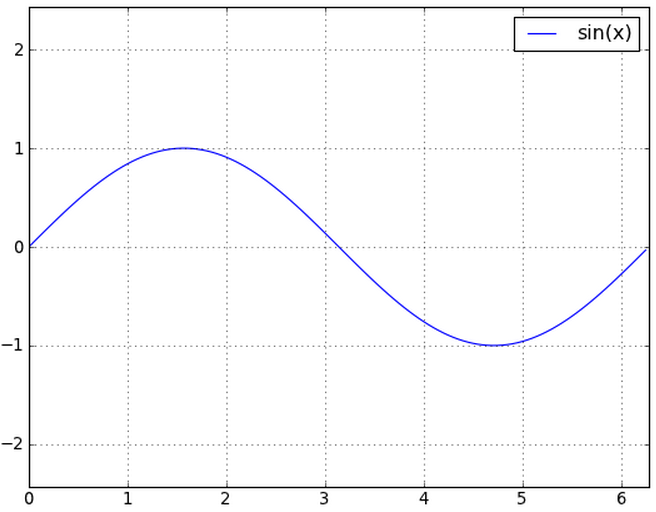
\includegraphics[width=0.53\textwidth]{img/plot9.png}
\end{center}
\vspace{-4mm}
\caption{Setting plot linits on the horizontal axis to $0$ and $2\pi$.}
\label{fig:plot9}
\vspace{-2mm}
\end{figure}
\noindent


\section{Plotting multiple functions at once}

This can be done very easily, just do not use the {\tt clf()}
command between the plots and you can have as many graphs 
in one figure as needed. Let us do three:

\begin{verbatim}
from numpy import *
from pylab import *
x = arange(0.5, 5, 0.05)
y1 = 1./x
y2 = 1. / (1 + x**2)
y3 = exp(-x)
axis=("equal")
clf()
plot(x, y1, label="y1")
plot(x, y2, label="y2")
plot(x, y3, label="y3")
legend()
lab.show()
\end{verbatim}
\noindent
The output is shown in Fig. \ref{fig:plot7}.
\newpage

\begin{figure}[!ht]
\begin{center}
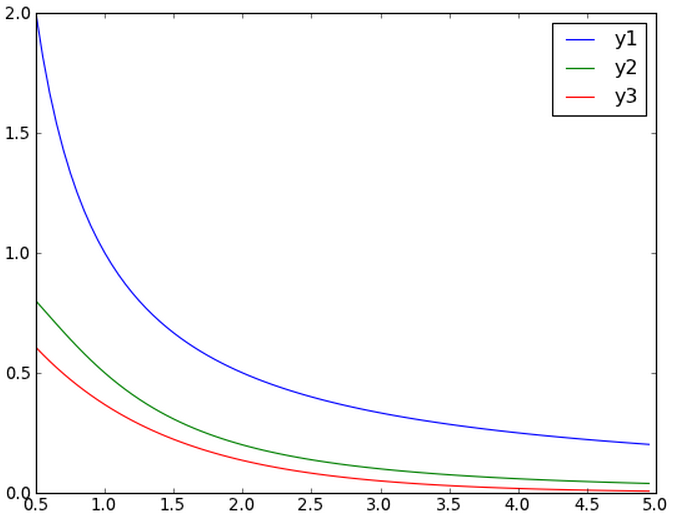
\includegraphics[width=0.55\textwidth]{img/plot7.png}
\end{center}
\vspace{-4mm}
\caption{Plotting graphs of functions $1/x$, $1 / (1 + x^2)$ and $e^{-x}$ in interval $(0.5, 5)$.}
\label{fig:plot7}
\end{figure}
\noindent
The {\tt plot()} command in Pylab is much more powerful, we just saw a small 
fraction of its functionality. For a complete list of options 
visit the Pylab page {\tt http:// www.scipy.org/PyLab}.

\section{Plotting parametric 2D curves}\label{subsec:planarcurves}

The concept of plotting based on two arrays of $x$ and $y$ coordinates
allows us to do much more than only plot graphs of functions of one variable.
We can easily plot more general curves such as circles, spirals and others.
Let us illustrate this on a spiral that this parameterized 
by 
$$
x(t) = t \cos(t), \ \ \ \ 
y(t) = t \sin(t)
$$ 
in the interval $(0, 10)$ for $t$. The complete code is

\begin{verbatim}
from pylab import *
from numpy import *
t = arange(0, 10, 0.05)
x = t*cos(t)
y = t*sin(t)
clf()
plot(x, y)
lab.show()
\end{verbatim}
The output is shown in Fig. \ref{fig:plot6}.

\newpage

\begin{figure}[!ht]
\begin{center}
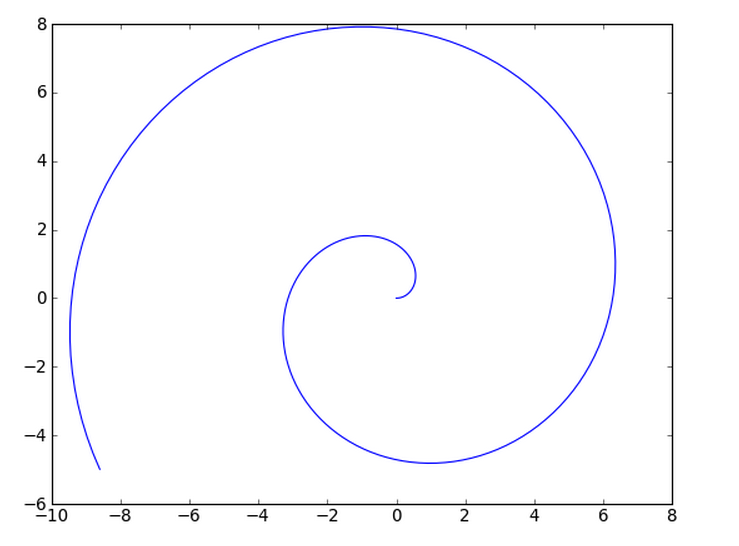
\includegraphics[width=0.6\textwidth]{img/plot6.png}
\end{center}
\vspace{-6mm}
\caption{Plotting a spiral.}
\label{fig:plot6}
\vspace{-0mm}
\end{figure}
\noindent

\section{Plotting parametric 3D curves}

For 3D plots it is practical to use the {\tt mplot3d} toolkit of the 
Python library Matplotlib. Let us begin with 
parametric 3D curves since this is analogous to how we handled planar curves in 
Subsection \ref{subsec:planarcurves}. 3D curves are sequences of 3D points
represented via three arrays of $x$, $y$ and $z$ coordinates, respectively. As an 
example we will plot the curve $x(t), y(t), z(t)$ where

$$
x(t) = (1 + t^2) \sin(2 \pi t), \ \ \ y(t) = (1 + t^2) \cos(2 \pi t), \ \ \ z(t) = t,
$$
and where the parameter $t$ lies in the interval $(-2, 2)$.

\begin{verbatim}
# Import Numpy and Matplotlib:
from numpy import *
import matplotlib as mpl
from mpl_toolkits.mplot3d import Axes3D
import matplotlib.pyplot as plt

# Set legend font size (optional):
mpl.rcParams['legend.fontsize'] = 15

# Setup the 3D plot:
fig = plt.figure()
ax = fig.gca(projection='3d')

# Define interval for parameter 't'
# and its division:
t = linspace(-2, 2, 100)

# Define the curve:
x = (1 + t**2) * sin(2 * pi * t)
y = (1 + t**2) * cos(2 * pi * t)
z = t

# Plot the curve
ax.plot(x, y, z, label='Parametric 3D curve')
ax.legend()

# Show the plot:
lab.show()
\end{verbatim}
The output is shown in Fig. \ref{fig:plot3d-1}.

\begin{figure}[!ht]
\begin{center}
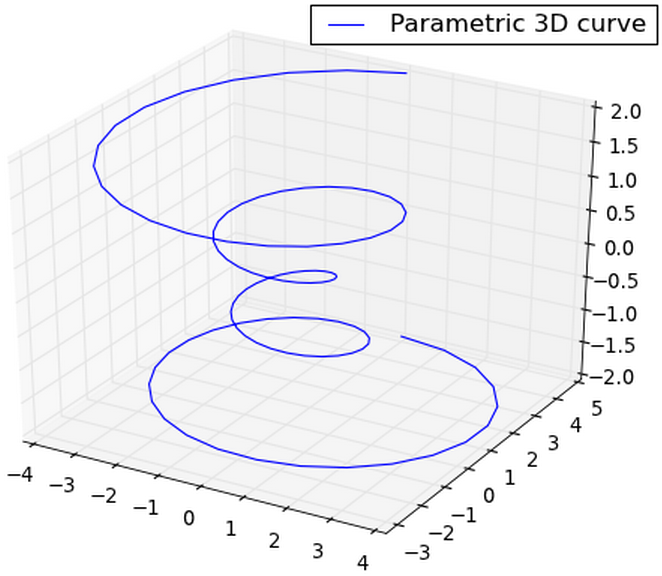
\includegraphics[width=0.6\textwidth]{img/plot3d-1.png}
\end{center}
\vspace{-4mm}
\caption{Plotting a parametric 3D curve.}
\label{fig:plot3d-1}
%\vspace{-1cm}
\end{figure}


\section{Plotting functions of two variables}

There are several ways to plot graphs of functions of two variables, 
first let us do this with Matplotlib's {\tt mplot3d} toolkit, then we will
use WebGL. We will plot the graph of the function 

$$
  f(x, y) = \sin(x) \sin(y)
$$
in the square $(-\pi, \pi) \times (-\pi, \pi)$.

\begin{verbatim}
# Import Numpy and Matplotlib:
from numpy import *
from mpl_toolkits.mplot3d import axes3d
import matplotlib.pyplot as plt

# Setup the 3D plot:
fig = plt.figure()
ax = fig.gca(projection='3d')

# Define intervals on the 'x' and 'y' axes
# and their divisions:
x = linspace(-pi, pi, 30)
y = linspace(-pi, pi, 30)

# Create Cartesian grid:
X, Y = meshgrid(x, y)

# Calculate values at grid points:
Z = sin(X) * sin(Y)

# Plot the data:
ax.plot_wireframe(X, Y, Z, rstride=1, cstride=1)

# Show the plot:
lab.show()
\end{verbatim}
The parameters {\tt rstride} (row stride) and {\tt cstride} (column stride)
can be used to make the plot coarser when they are set to 2, 3, etc.
The output is shown in Fig. \ref{fig:plot3d-2}.

\begin{figure}[!ht]
\begin{center}
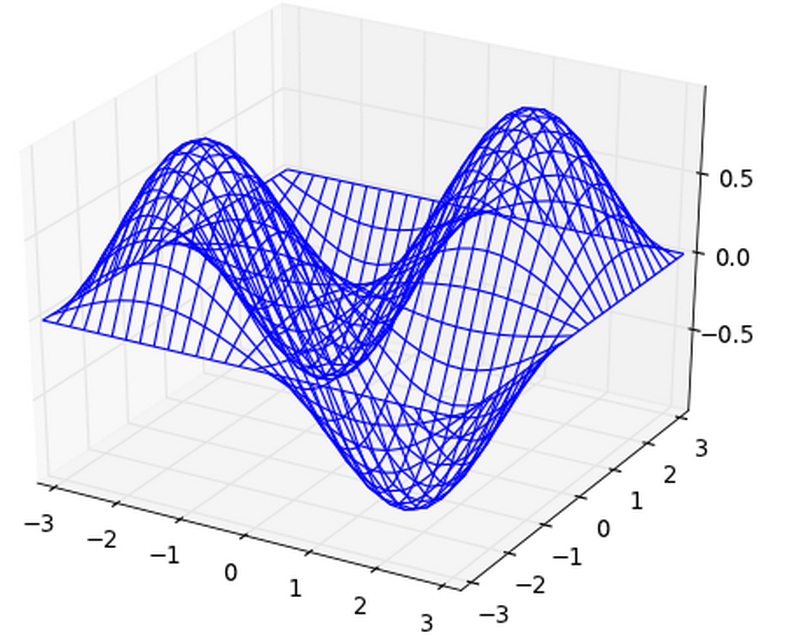
\includegraphics[width=0.6\textwidth]{img/plot3d-2.png}
\end{center}
\vspace{-4mm}
\caption{Wireframe plot of the function $f(x, y)$.}
\label{fig:plot3d-2}
%\vspace{-1cm}
\end{figure}
\noindent
Solid surface plot can be obtained by replacing in the above code 
{\tt plot\_wireframe} with {\tt plot\_surface}. 
The output is shown in Fig. \ref{fig:plot3d-3}.

\begin{figure}[!ht]
\begin{center}
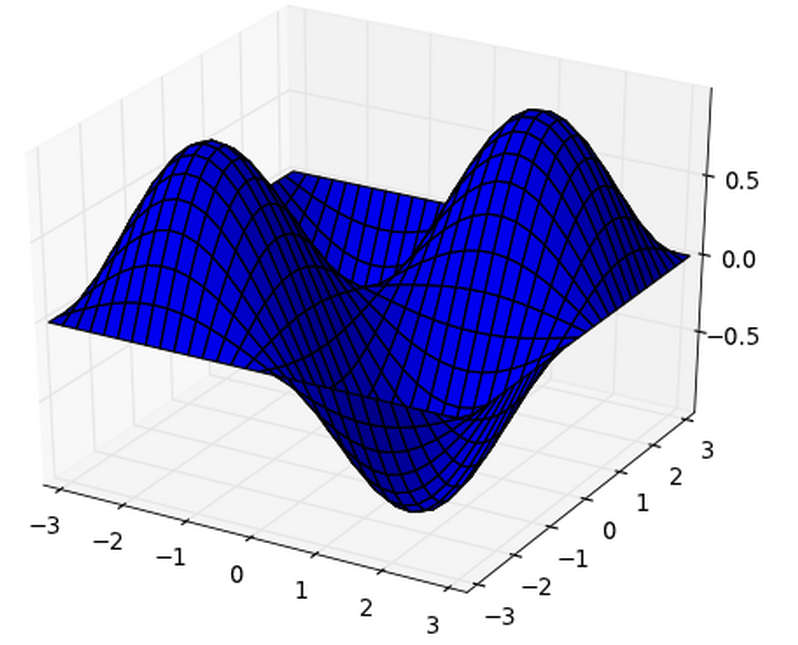
\includegraphics[width=0.6\textwidth]{img/plot3d-3.png}
\end{center}
\vspace{-4mm}
\caption{Surface plot of the function $f(x, y)$.}
\label{fig:plot3d-3}
%\vspace{-1cm}
\end{figure}
\newpage

\noindent
Contour plot can be obtained by replacing in the above code 
the line 

\begin{verbatim}
ax.plot_wireframe(X, Y, Z, rstride=1, cstride=1)
\end{verbatim}
with 

\begin{verbatim}
cset = ax.contour(X, Y, Z)
ax.clabel(cset)
\end{verbatim}
The output is shown in Fig. \ref{fig:plot3d-4}.
\newpage

\begin{figure}[!ht]
\begin{center}
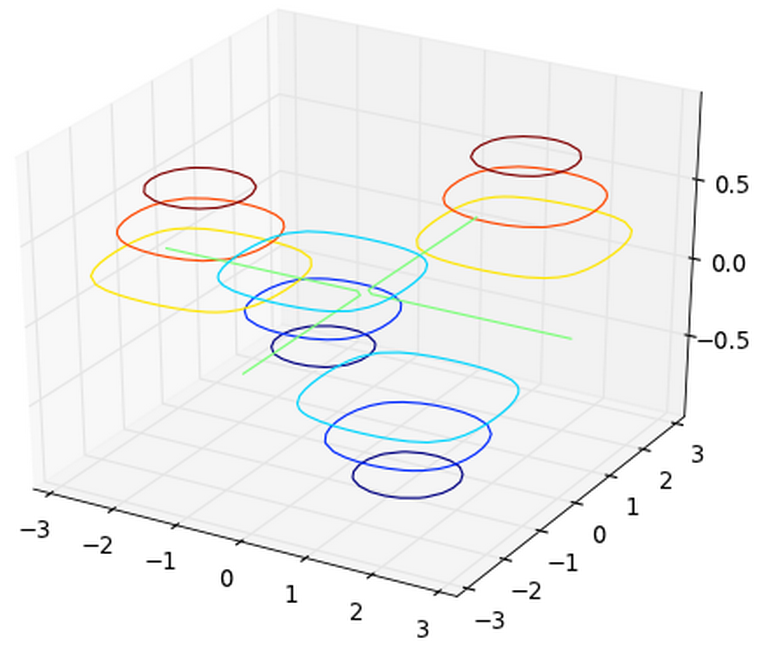
\includegraphics[width=0.6\textwidth]{img/plot3d-4.png}
\end{center}
\vspace{-4mm}
\caption{Contour plot of the function $f(x, y)$.}
\label{fig:plot3d-4}
%\vspace{-1cm}
\end{figure}
\noindent
We have only mentioned the most basic Matplotlib's functionality, for more options 
we refer to the tutorial 
at {\tt http://matplotlib.sourceforge.net/mpl\_toolkits/mplot3d}.


\section{Plotting functions of two variables with WebGL}

For this functionality, your browser has to support WebGL (most of modern browsers do, 
with the exception of Internet Explorer). See the introductory tutorial {\em Welcome to NCLab}
on the page {\tt http://femhub.com/ nclab-tutorials/} for detailed instructions on how to enable WebGL. 
In the following example, we plot the graph of the function 

$$
  f(x, y) = \sin(\sqrt{x^2 + y^2})
$$
in the square $(0, 10) \times (0, 10)$.

\begin{verbatim}
from numpy import sin, sqrt, arctan

# Define intervals on the x and y axes.
x0 = 0.0
x1 = 10.0
y0 = 0.0
y1 = 10.0

# Define the corresponding divisions.
nx = 100
ny = 100

# Define a function:
def f(x, y):
    return sin(sqrt(x**2 + y**2))

# Render the surface using WebGL.
lab.surface((x0, x1, nx), (y0, y1, ny), f)
\end{verbatim}
The output is shown in Fig. \ref{fig:webgl}.

\begin{figure}[!ht]
\begin{center}
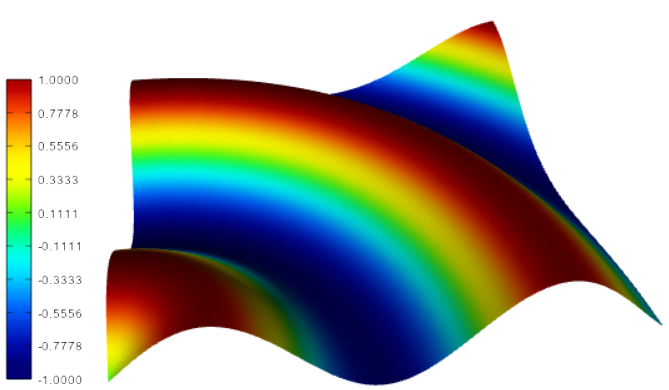
\includegraphics[width=0.8\textwidth]{img/webgl.png}
\end{center}
\vspace{-2mm}
\caption{Plotting functions of two variables with WebGL.}
\label{fig:webgl}
%\vspace{-1cm}
\end{figure}





\end{document}
